\section{Bus Fabric and Memory Subsystem}

Bus fabric is digital plumbing. A master, such as a processor, requests a read or write on some address; the bus fabric routes the request to the correct slave device, and routes the response back. RISCBoy implements two bus fabric standards:

\begin{itemize}
\item AMBA 3 AHB-Lite connects masters to high-performance devices such as SRAM controllers
\item AMBA 3 APB connects to simple devices such as a UART
\end{itemize}

Figure \ref{diagram:crossbar_structure} shows the structure of the AHB-Lite crossbar ({\tt ahbl\_crossbar.v}). The crossbar is shown in context in figure \ref{diagram:system_arch}. An independent AHB-Lite datapath connects each of $m$ masters to each of $n$ slaves. One master can address one slave at a time, and one slave can be in data-phase with one master at a time; subject to these constraints, up to $\min(m,n)$ independent transfers can take place in a single machine clock cycle.

Some claim AHB-Lite does not "support" multi-master arbitration. Their problem is a lack of enthusiasm: motorbikes do not "support" wheelies by design, but are excellent at it.

\begin{figure}[!htb]
\centering
\caption{AHB-Lite crossbar, module-level block diagram} 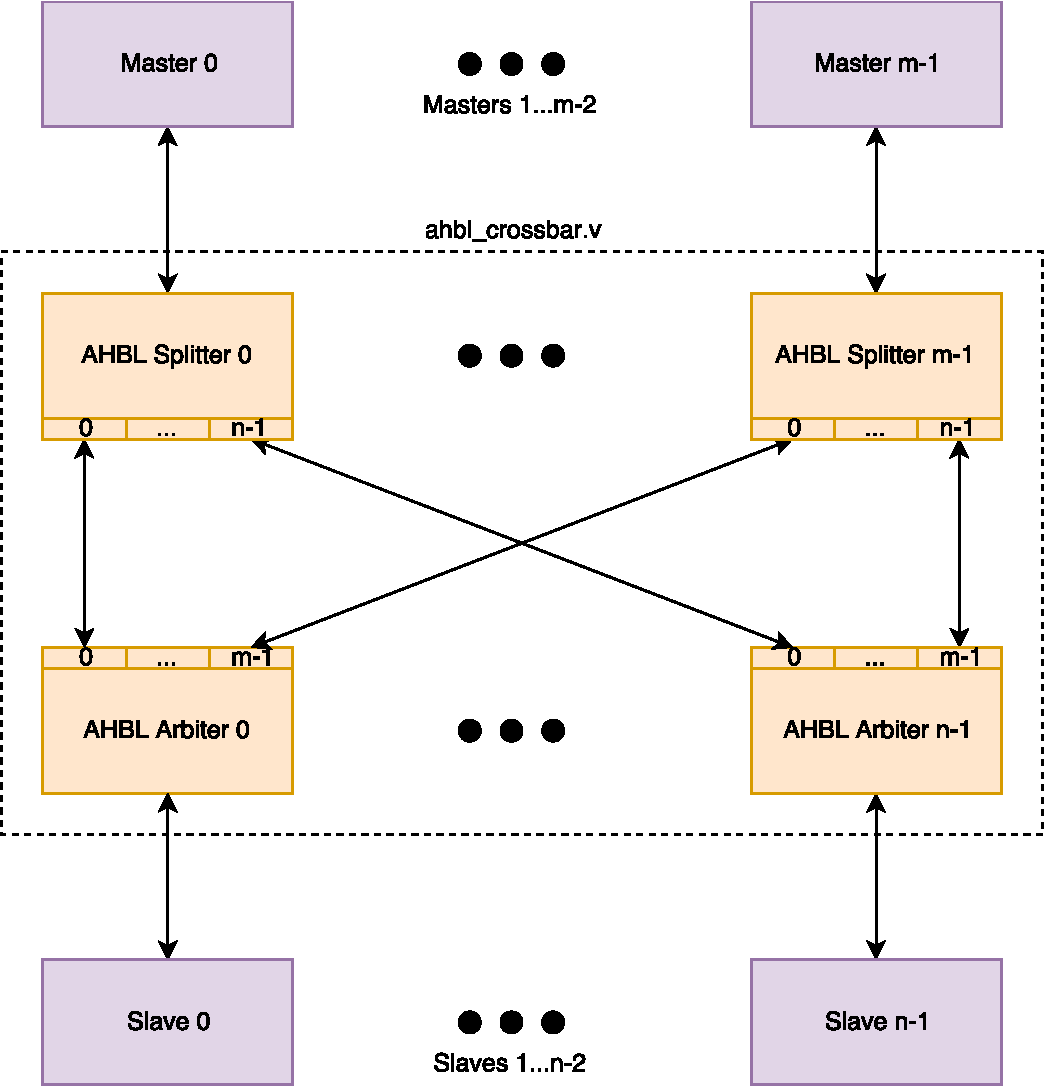
\includegraphics[width=0.6\textwidth]{diagrams/crossbar_structure.pdf}
\label{diagram:crossbar_structure}
\end{figure}

Each master is under the illusion that it is the only master in the system, but that slaves sometimes take longer to respond. During this waiting period, the slave may actually have fielded multiple transactions from higher-priority masters; this interaction is handled by the slave's AHB-Lite arbiter, and is transparent to the masters.

One of the crossbar's slave ports is attached to an AHBL-APB bridge. This bridge appears as a slave to the AHB portion of the bus fabric, and as a master to the APB portion. There are three main benefits to this scheme:

\begin{itemize}
	\item APB is fundamentally simpler
	\begin{itemize}
		\item This keeps peripheral gate count down
		\item The peripherals on the APB bus do not need the full AHB-Lite bandwidth anyway
	\end{itemize}
	\item Fewer AHB-Lite slaves
	\begin{itemize}
		\item There is a nonlinear area scaling associated with adding slaves to the AHB-Lite fabric
		\item This would also add extra gate delays to a fairly critical data path
	\end{itemize}
	\item One APB master
	\begin{itemize}
		\item AHB-Lite masters get arbitrated down to one inside the AHB-Lite crossbar. APB slaves do not care who is addressing them.
		\item Different masters accessing different APB slaves will have to queue to use the bridge, even though they could theoretically proceed simultaneously
		\item However, area/complexity vs performance tradeoff is more than worth it for slow peripherals
		\item Multi-master APB is easy to implement, but never used in practice, due to the above tradeoff
	\end{itemize}
\end{itemize}

The splitter and arbiter modules in the AHB-Lite crossbar can also be used on their own. Arbitrary multi-layer busfabric topologies should be possible with these two components.

Currently, the RISCBoy busfabric does not support AHB-Lite bursts (TODO), and the masters do not use them.

\subsection{AHB-Lite Primer}

For a full understanding of the bus standard used by RISCBoy, read through ARM's AMBA 3 AHB-Lite spec. This document is mirrored in the {\tt reference} folder in the GitHub repository, and gives a clear and comprehensive breakdown of AHB-Lite. However, the following overview should provide sufficient understanding of the standard to read through the Verilog.

Transactions take place in two phases, named the address phase and the data phase. During the address phase, the master asserts signals which control the nature of the transfer, such as the address, whether the transfer is a read or write, protection/permission information, the width of the data, and so on. During the data phase, data is asserted on either the read or write data bus ({\tt hrdata} and {\tt hwdata}), but never both. {\tt hrdata} is driven by the slave, and {\tt hwdata} by the master.

The central conceit of AHB-Lite is that these two phases are {\it pipelined}. Whilst the master is asserting or accepting data for an earlier transaction (currently in data phase), it concurrently asserts address and control information for a later transaction (currently in address phase). As is generally the case with pipelining, the goal is to enable higher clock frequencies with undiminished work-per-clock.

\begin{figure}[H]
\centering
\caption{AHB-Lite transfers, a simple example}
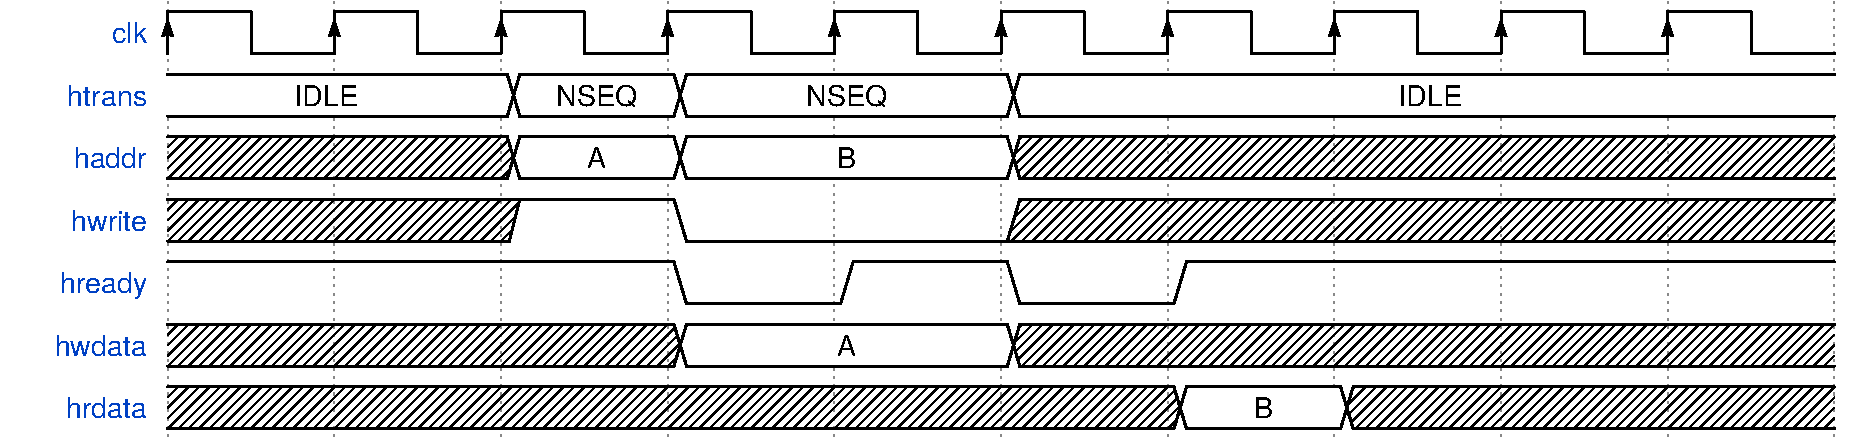
\includegraphics[width=0.9\textwidth]{waves/ahbl_basic.pdf}
\label{diagram:ahbl_basic}
\end{figure}

In figure \ref{diagram:ahbl_basic}, a master carries out two AHB-Lite transactions: a write to address A, followed by a read from address B. Only a subset of AHB-Lite signals are shown on the diagram. {\tt htrans}, {\tt haddr}, and {\tt hwrite} are driven by the master, during the address phase; the other two are data phase signals. {\tt htrans} indicates the type of transfer the master next wishes to perform, which is one of {\tt IDLE}, {\tt NSEQ} (non-sequential), {\tt SEQ} and {\tt BUSY}. The latter two are exclusive to burst transactions, which are not used in RISCBoy. (See the ARM spec if you do want details.)

Sometimes a slave is unable to service a request immediately, as shown in figure \ref{diagram:ahbl_basic_stall}. {\tt hready} is a data phase signal, which signifies the end of the current data phase.

\begin{figure}[H]
\centering
\caption{AHB-Lite transfers, simple example with stalling}
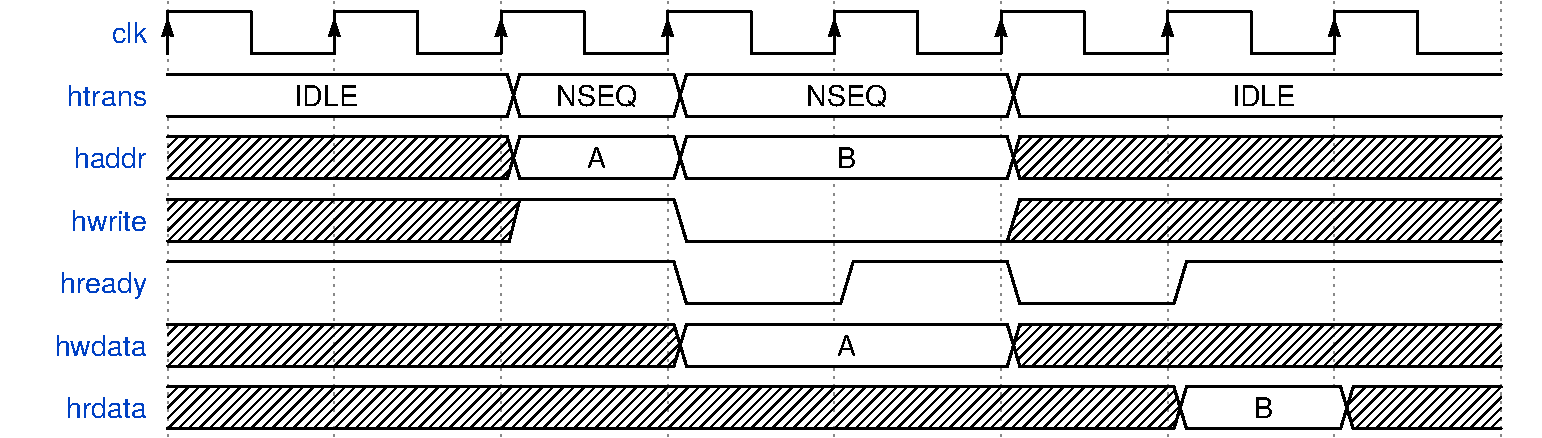
\includegraphics[width=0.9\textwidth]{waves/ahbl_basic_stall.pdf}
\label{diagram:ahbl_basic_stall}
\end{figure}

This slave needs two cycles to perform each data phase; perhaps it is an SRAM capable of running only at half the system clock speed. Therefore, {\tt hready} is low for one cycle, and high for the second (last) cycle of each data phase. The master drives {\tt hwdata} for the duration of A's data phase, waiting for the slave to signal completion. {\tt hrdata}, on the other hand, is invalid until the final cycle of a read data phase.

Note that an address phase does not complete until the preceding transfer's data phase completes. In figure \ref{diagram:ahbl_basic_stall}, address B (and associated address-phase signals) continue to be driven until the A data phase completes. {\tt IDLE} transactions do have a data phase, which always completes immediately. Consequently, {\tt hready} idles high while the bus is in an idle state. This is why A's address phase completes immediately in the figure.

In a practical system, there are multiple slaves. Each drives a signal called {\tt hreadyout}, to indicate that {\it that slave} is ready. The bus fabric tracks which slave the master is currently accessing in the data phase, and selects that slave's {\tt hreadyout} to be the global {\tt hready}. To see why this is necessary, think about the situation where a master is in data phase with one slave, and address phase with a different slave.

\subsection{Multi-Master Operation}

In a single-master busfabric, {\tt hready} is a global signal, which causes the entire AHB-Lite state machine (masters, slaves, fabric, the lot) to advance. Where multiple masters are concerned, {\tt hready} is more subtle; in part it is a per-master stall signal. At this point we need to be more specific about the relationship between {\tt hreadyout} and {\tt hready}.

Any AHB-Lite slave port (of which there is one on the master side of the splitter, $n$ on the master side of the arbiter, and one on each slave device) has an output called {\tt hreadyout}, which indicates the slave's readiness. Each of these ports also has an input called {\tt hready}, which indicates that the data phase is ending for the master who is connected to this slave (which does not mean that it is in data phase with {\it this} slave; it may be addressing this slave while in data phase with another). {\tt hready} is a function of {\tt hreadyout}s and bus state. The connections between masters, splitters, arbiters and slaves are shown in figure \ref{diagram:crossbar_structure}.

In the single-layer crossbar on RISCBoy, each system AHB-Lite slave is the slave of an arbiter, which is the slave of several splitters, each of which is the slave of a system master. As a general rule, the busfabric must filter system slaves' {\tt hreadyout}s up to each system master, tie {\tt hreadyout}s across to {\tt hready}s at the very top of the busfabric, and then distribute these {\tt hready} signals down to the correct system slaves.

\subsubsection{Multiple Masters, One Slave}

The arbiters are the most complex busfabric component, so it is instructive to consider interactions between multiple masters and a single slave, which are mediated by one arbiter. There are additional complexities when we combine arbiters and splitters to build a crossbar, which are discussed in the next section.

In figure \ref{diagram:ahbl_mm_simult1}, two masters attempt to access a single slave simultaneously. Assume that master 0 always wins address-phase arbitration:

\begin{figure}[H]
\centering
\caption{AHB-Lite transfers, two masters access one slave}
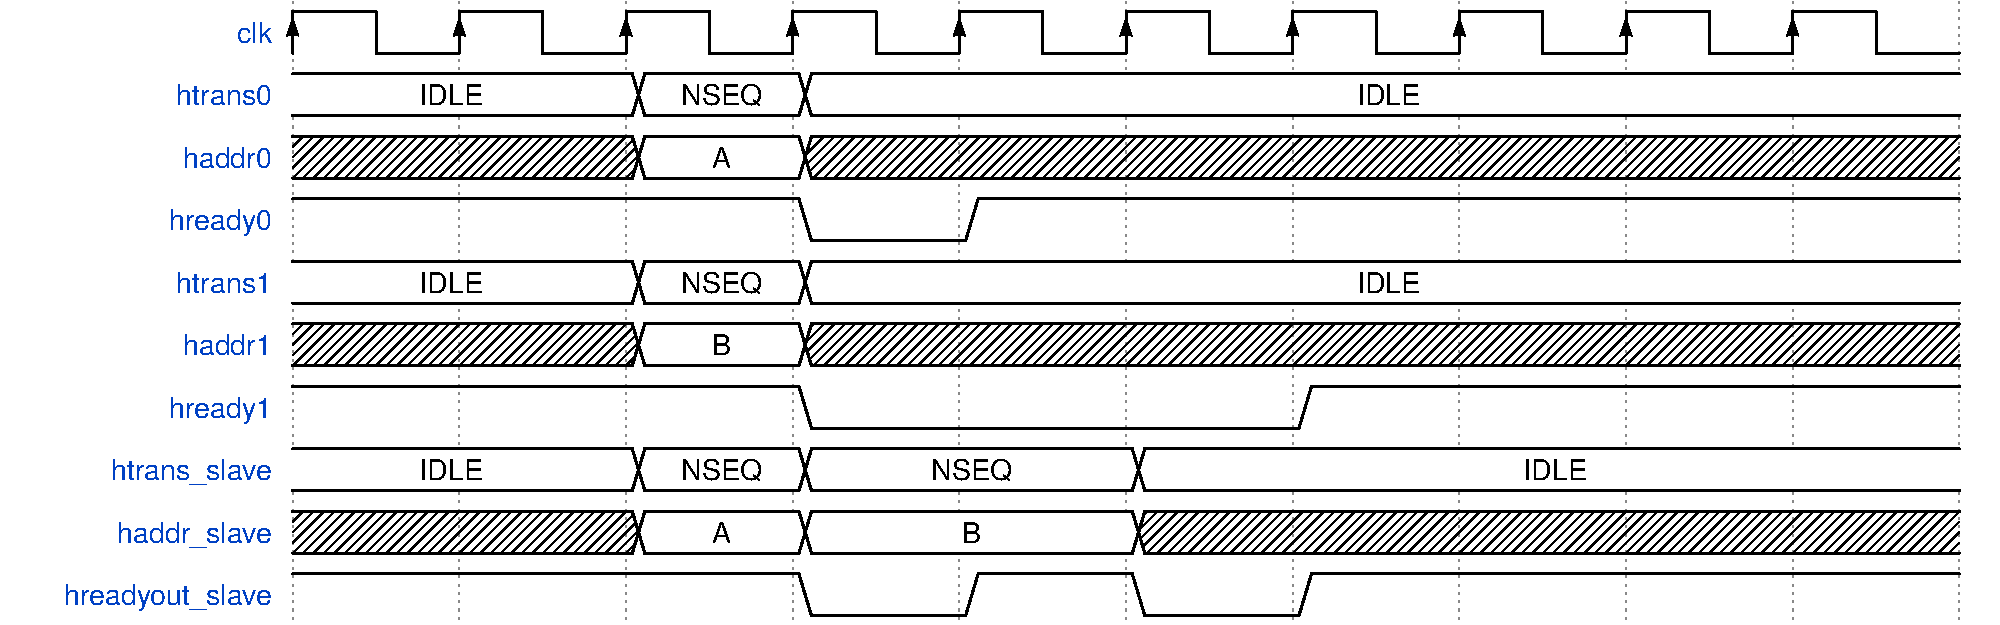
\includegraphics[width=0.9\textwidth]{waves/ahbl_mm_simult1.pdf}
\label{diagram:ahbl_mm_simult1}
\end{figure}

Again, we assume the slave requires 2 cycles to complete each data phase.

If we look at each master's trace, there is no indication at all that there is more than one master in the system: they present an address, and subsequently the transaction completes. Likewise, the slave neither knows nor cares that there are multiple masters: it simply carries out transactions according to the address-phase signals it sees. All of the smoke, mirrors and machinery are inside of the arbiter.

One odd feature of this trace is that, when the slave sees the address B, no master is asserting this address.

\begin{enumerate}
	\item Initially, both masters assert {\tt IDLE}; {\tt IDLE} data phases complete in one cycle
	\item {\tt IDLE} data phases are concurrent with A, B address phases, so these {\it also} complete immediately
	\item From the master 1's point of view, transaction B proceeds immediately to data phase.
	\item From both the master 0's and the slave's point of view, transaction A proceeds immediately to data phase
	\item Whilst the slave is in data phase for A, it is simultaneously in address phase for B
	\item When A data phase completes, master 0 is signaled, and B proceeds to data phase at the slave
	\item When B data phase completes, master 1 is signaled
\end{enumerate}

More concisely put, the first clock cycle of a given transaction's data phase may differ between the slave and master, but the {\it last} cycle of that data phase is always the same clock cycle. The slave address phase will occur some time between the master address phase starting, and the slave data phase starting. These are strong enough guarantees for correct operation.

Based on this discussion, the AHB-Lite arbiters need the facility to buffer one address-phase request, per master. A buffered request will be applied before any new requests from that master, but after any higher-priority requests. There is a nonzero hardware cost to this buffering, but there are clear engineering benefits to keeping this complexity confined to the arbiters, as they are the only component in the busfabric which is explicitly "multi master".

\begin{figure}[H]
\centering
\caption{AHB-Lite transfers, two masters access one slave, with low-priority back-to-back}
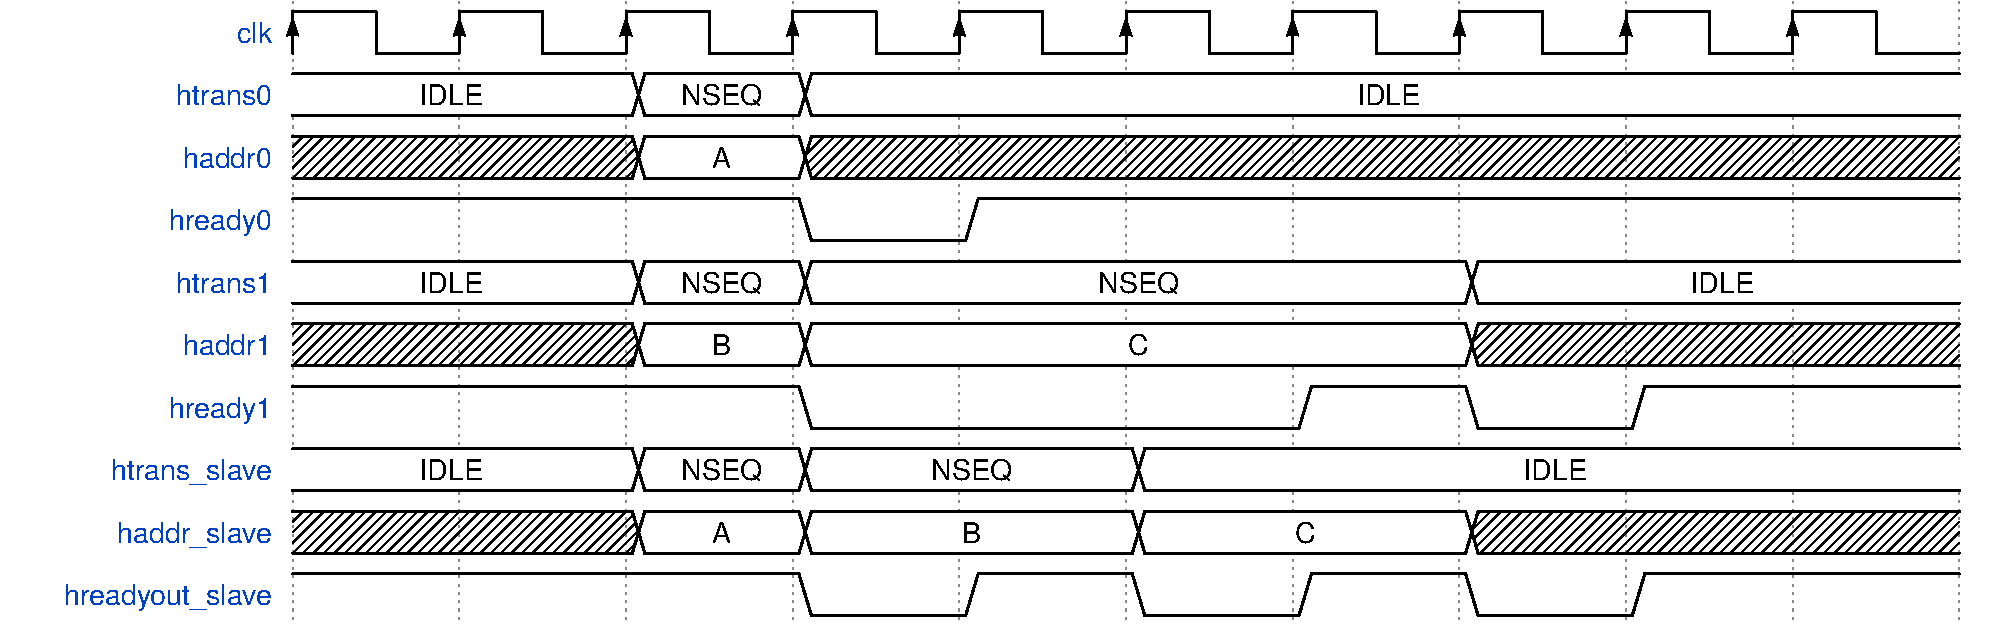
\includegraphics[width=0.9\textwidth]{waves/ahbl_mm_simult2.pdf}
\label{diagram:ahbl_mm_simult2}
\end{figure}

Figure \ref{diagram:ahbl_mm_simult2} shows the same sequence of events as figure \ref{diagram:ahbl_mm_simult1}, except master 1 now performs two back-to-back transactions. Once B's slave address phase completes, the arbiter's request buffer is cleared, and the C request passes transparently through the arbiter to the slave. Again, the only indication to master 1 of any master 0 activity is increased latency.

There is a different case which requires the arbiter's request buffer, shown in figure \ref{diagram:ahbl_mm_simult3}.

\begin{figure}[H]
\centering
\caption{AHB-Lite arbiter: simultaneous request buffer writes}
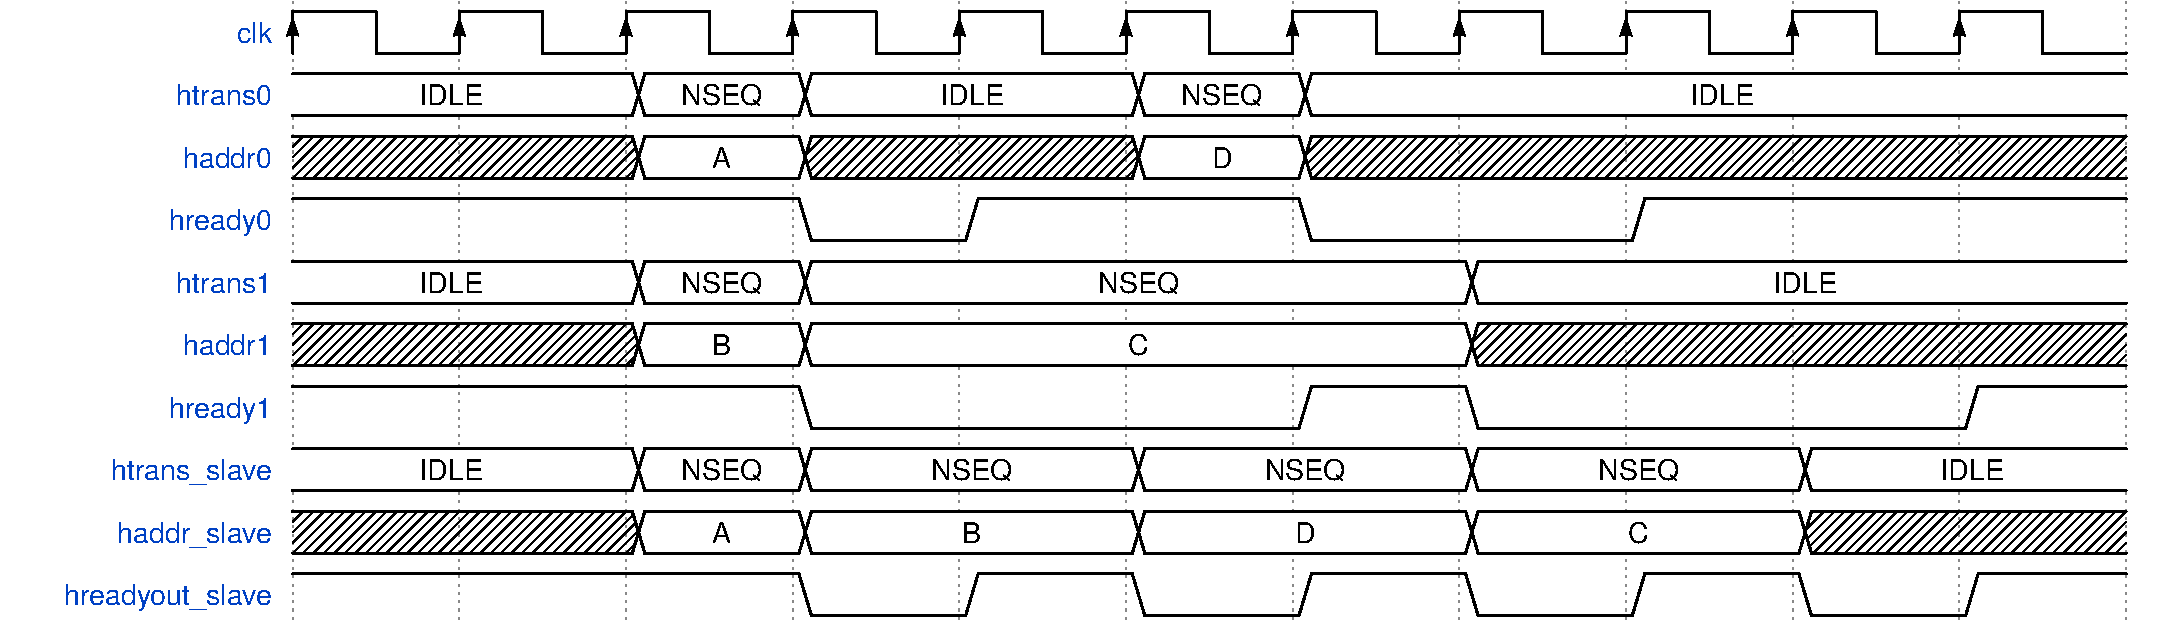
\includegraphics[width=0.9\textwidth]{waves/ahbl_mm_simult3.pdf}
\label{diagram:ahbl_mm_simult3}
\end{figure}

At the instant where D address phase is asserted, {\tt hready0} is high, because master 0 previously asserted an {\tt IDLE} transfer. However, the slave is not ready. In this case, the arbiter needs to buffer master 0's request, even though it is the highest-priority master. The buffered request is cleared once its slave address phase completes, as usual.

On the next cycle, B's data phase completes, and master 1 also considers this to be the end of the C address phase. The arbiter must write the C request into master 1's request buffer. Master 0's buffered request will continue to take priority over master 1's buffered request, until the first buffer is cleared.

There is one final case, for two masters accessing one slave, which is worth being aware of (figure \ref{diagram:ahbl_mm_latearrival}).

\begin{figure}[H]
\centering
\caption{AHB-Lite arbiter: late arrival of high priority request}
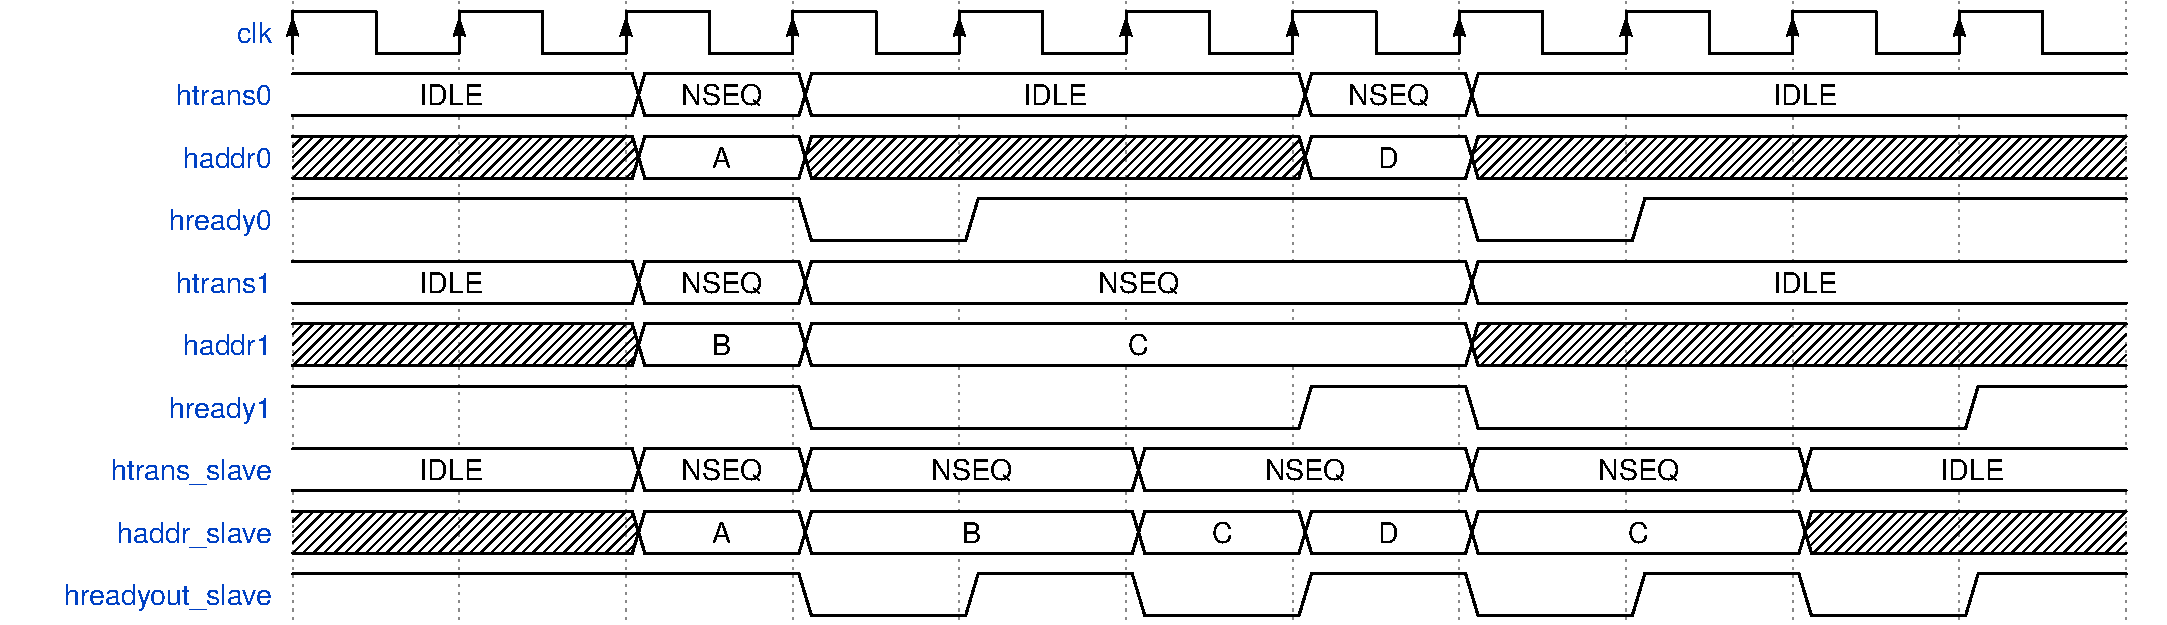
\includegraphics[width=0.9\textwidth]{waves/ahbl_mm_latearrival.pdf}
\label{diagram:ahbl_mm_latearrival}
\end{figure}

Whilst {\tt hreadyout} is low, the C address briefly appears on the slave bus, before being replaced by the higher-priority D request. \textbf{This is a departure from the AHB-Lite standard}, which stipulates the address must be constant during this time. This is deliberate, and easily amended. Slaves are generally insensitive to address-phase request during this time (as there is no performance benefit to latching APR before {\tt hreadyout}, due to the way the bus operates), and this avoids a priority inversion, reducing average latency for higher-priority masters. If you find something that this breaks, write me an angry email! I would be interested to see such a slave.

The D request causes the low-priority C request to be buffered; the B data phase completes on this cycle, hence, from master 0's point of view, the C address phase does too.

\subsubsection{Full Crossbar}

The previous section discussed some cases where multiple masters access a single slave, and showed how the arbiter safely navigates them. There are yet more issues to consider when multiple masters and multiple slaves are involved, which must be handled without added latency cycles, and with minimal extra gate delay.

For example, a master may be engaged in address phase with one arbiter and data phase with another arbiter simultaneously, via a splitter, and these two arbiters will not necessarily signal {\tt hreadyout} at the same time. Consequently, a master may have a positive {\tt hready}, filtered from its data phase arbiter, when its address phase arbiter has a negative {\tt hreadyout}, which requires action on the arbiter's part.

There is also the issue that being in data phase with an arbiter does not mean you are genuinely in data phase with the arbitrated slave; in fact, a very simple sequence of events (all masters {\tt IDLE} $\to$ all masters {\tt NSEQ}) will put all masters simultaneously in data phase with the same arbiter. The arbiter behaviour described in the previous section should allow us to abstract this away, provided we can deal with the first issue safely.

Splitters will filter their slaves' {\tt hreadyout}s based on which is currently in data phase, and present it on their own slave port. Arbiters will present their slave's {\tt hreadyout} on any master-facing ports which are in data phase with the arbiter, and will present ${\tt hreadyout} = 1$ on any idle ports.

Splitters will fan their {\tt hready} signal out to all of their slaves; a low {\tt hready} directed at a slave you are not engaged with is harmless.

\subsection{Memories}

RISCBoy possesses two memory areas for data and code: an external SRAM (512 kiB, 16 b wide, asynchronous), and internal RAM (8 kiB, 32 b wide, synchronous), assembled from FPGA block RAMs. The former is the main system memory, which most games will simply load into as a flat image; the latter is intended to be used for processor stack, and some critical code sections, including ISRs. Internal RAM also contains the first-stage bootloader, as it can be initialised during FPGA configuration, so is a convenient place to put the first few thousand instructions the processor will execute at start-of-day. SRAM was chosen for the external memory due to the low initial access latency -- this permits reasonable performance without building complex cache hierarchies into the system bus masters. On a larger FPGA we could consider something like HyperRAM, or even DDRx SDRAM.

Both memories need to be interfaced to the AHB-lite system bus. SRAMs aren't too complex, but they can be a little fiddly to use efficiently due to the timing of AHB-lite -- in particular, the alignment of {\tt haddr} and {\tt hwdata} is more or less the opposite of what you want for a synchronous SRAM.

The internal SRAM can perform one 32-bit read or write per cycle. The external SRAM can also service a 32-bit AHB-lite read every cycle, because it is double-pumped; the controller performs two back-to-back 16 bit SRAM reads in one clock cycle. However, writes to external SRAM are limited to 16 bits per clock cycle, due to the timing of the {\tt WE} pin, which is deasserted part way through each access. This is reasonable -- reads are more common than writes, for almost any workload. However, special cases like the processor stack will benefit from the improved write performance of IRAM.

\subsubsection{Internal RAM}

Synchronous SRAMs typically behave as follows (ignoring details such as transparency):

\begin{itemize}
	\item Address, write data and write enable are presented on one clock
	\item Read data is available on the next clock (and the whole process is pipelined)
	\item Byte-enables allow narrow writes to be performed without a read-modify-write sequence.
\end{itemize}

This is shown in figure \ref{diagram:sync_sram_only}. However, in AHB-lite, read and write data are both presented during the data phase, which begins on the cycle after the address phase completes. The timing of this is shown in figure \ref{diagram:sync_sram_ahb_access}. Note the difference in timing between {\tt wdata} in figure \ref{diagram:sync_sram_only} and {\tt hwdata} in figure \ref{diagram:sync_sram_ahb_access}.


\begin{figure}[H]
\centering
\caption{Timing of synchronous SRAM interface}
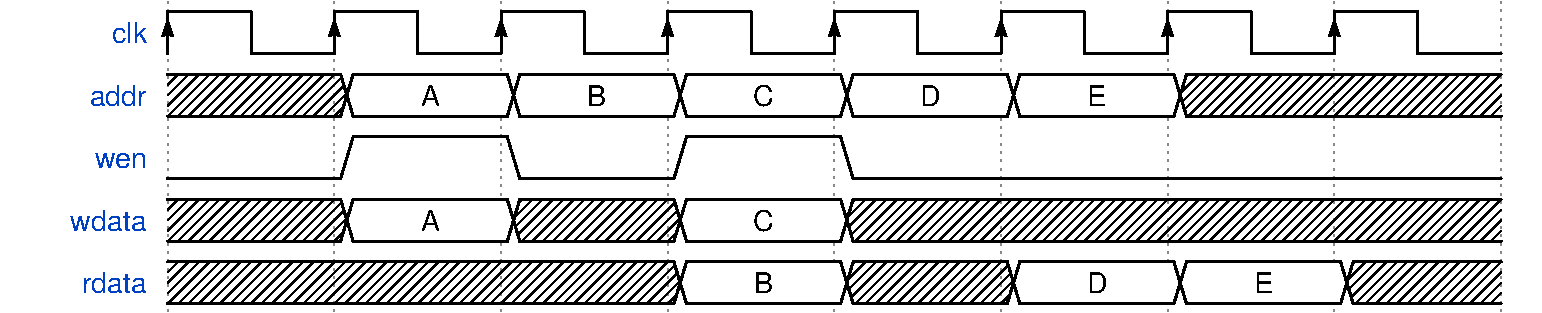
\includegraphics[width=0.7\textwidth]{waves/sync_sram_only.pdf}
\label{diagram:sync_sram_only}
\end{figure}


\begin{figure}[H]
\centering
\caption{Timing of AHB-lite SRAM accesses, showing write data misalignment}
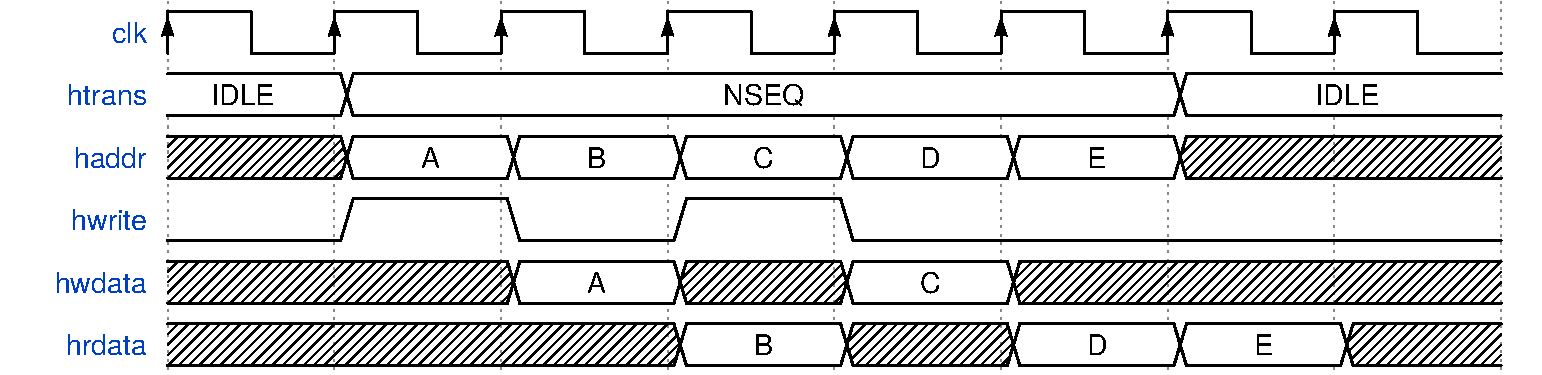
\includegraphics[width=0.7\textwidth]{waves/sync_sram_ahb_access.pdf}
\label{diagram:sync_sram_ahb_access}
\end{figure}

The issue is that, as we can't source signals from the future, the SRAM write cycle muust be delayed so that write address is aligned with write data. However, if the next transfer is a read, there is a collision: the delayed write address would need to be presented on the same cycle as the read address, which is impossible for a single-port SRAM. One way to resolve this is to simply insert wait states on write access, shown in figure \ref{diagram:sync_sram_ahb_stall}.

\begin{figure}[H]
\centering
\caption{AHB-lite SRAM access: resolving address collision with wait states}
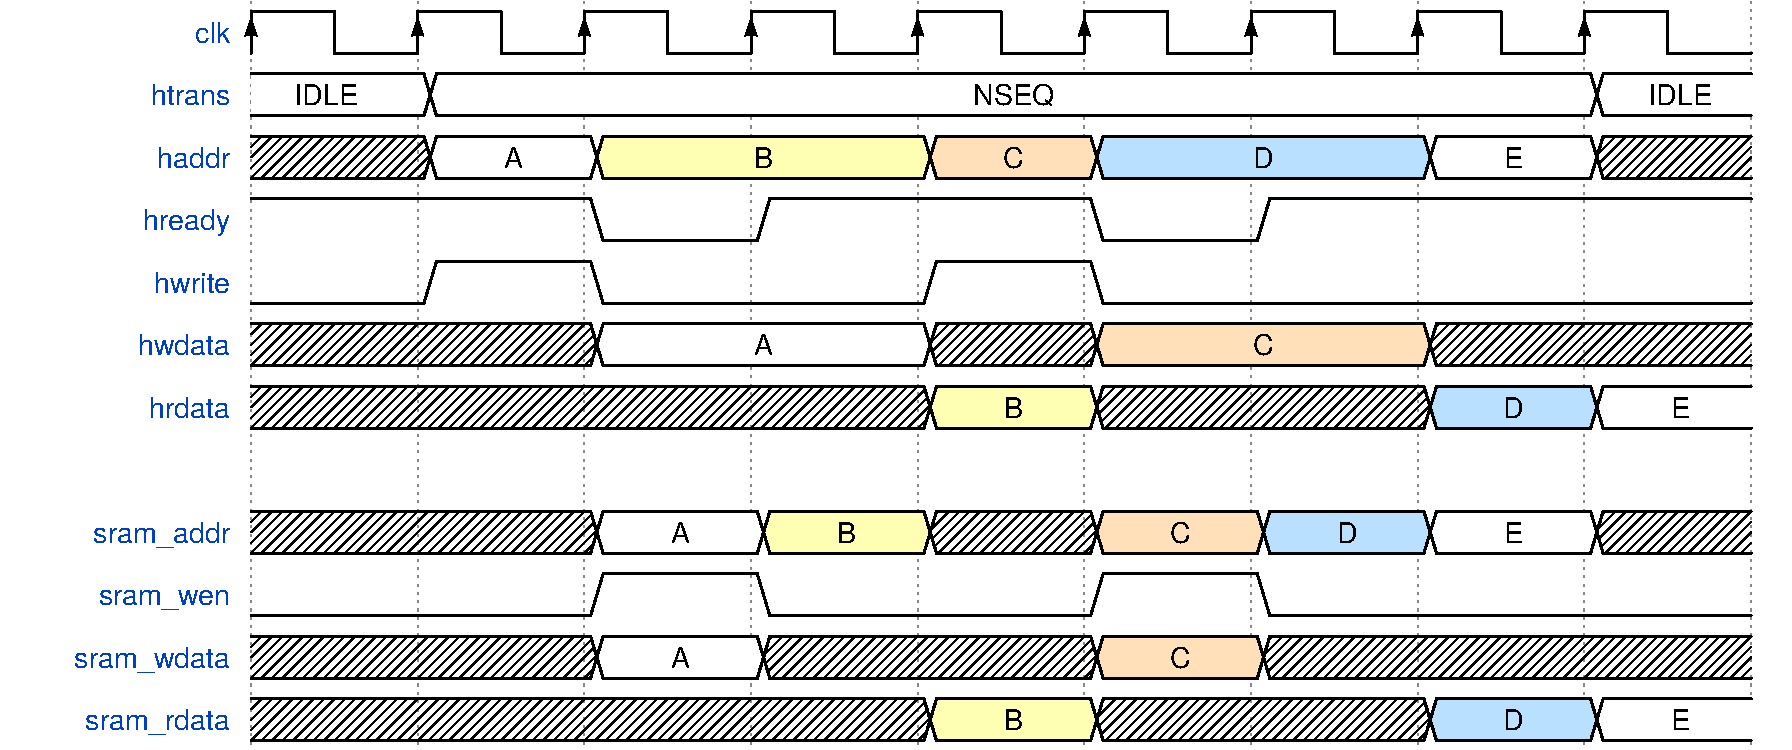
\includegraphics[width=0.76\textwidth]{waves/sync_sram_ahb_stall.pdf}
\label{diagram:sync_sram_ahb_stall}
\end{figure}

This works, but the performance cost is significant if you are constantly swapping back and forth between reads and writes (like, say, a processor!). This needn't be so. Noting that:

\begin{itemize}
	\item Multiple consecutive writes can proceed fine; all of their addresses are delayed, so there is no overlap
	\item Write-to-read has a single collision, and no more
	\item Consecutive reads are also fine
	\item A run of consecutive reads is always followed by either an idle cycle or a write cycle
\end{itemize}

We can surmise that there will never be more than one write pending at a time, and we will {\it always} eventually get a chance to commit that write to SRAM, even if traffic is completely back-to-back.

\subsubsection{Main Memory}

TODO